\documentclass[10pt,a4paper]{report}
\usepackage[utf8]{inputenc}
\usepackage{amsmath}
\usepackage{amsfonts}
\usepackage{amssymb}
\usepackage{fancyhdr}
\usepackage{tikz}

\usetikzlibrary{positioning, arrows, backgrounds, fit}
\usepackage{titlesec, blindtext, color}
\newcommand{\hsp}{\hspace{20pt}}
\titleformat{\chapter}[hang]{\Huge\bfseries}{\thechapter\hsp}{0pt}{\Huge\bfseries}

\begin{document}
\chapter{Augmented Chess:\\ Assignment 5}

\begin{center}
{\Large \textbf{Group Members}}

\begin{tabular}{l r}
Jacob Holm Mortensen		&	jmorte14@student.aau.dk\\
Martin Raunkjær Andersen	&	marand13@student.aau.dk\\
Thomas Gwynfryn McCollin	&	tmccol14@student.aau.dk
\end{tabular}
\end{center}

\subsection*{Question 2}
\begin{quote}
	\textit{From the characteristics mentioned in Section 8.1 of “Engineering Web Applications”, which ones are relevant for your Web application? Why?}
\end{quote}

The primary quality requirement of AugmentedChess are as follows.
\begin{enumerate}
	\item Usability
	\item Portability
	\item Reliability
\end{enumerate}
These requirements are based of the definition in Section 8.1 of “Engineering Web Applications”. AugmentedChess is a game and therefore the primary factor retaining users is the entertainment value of the application. A high usability ensure that the application can be easily used by the users with minimal extra effort. Secondly portability and compatibility with as many different platforms as possible supports the ease of using the application. Finally, some features of AugmentedChess require consistent up-time in order to provide worthwhile entertainment. These features are the multi-player aspects that we hope to include in the application. If two players are constantly disconnected from each other, before the game can be resolved then both will look for different entertainment venues.

\subsection*{Question 3}
\begin{quote}
 \textit{For the answer to the previous question, describe your plan to test that those characteristics are ensured.}
\end{quote}

In order to answer this question we will propose a test for each of the quality requirements.
\subsubsection*{Usability}
To adequately test the usability of the application we would conduct a series of user tests. These tests would consist of members of our target audience i.e. chess players. This is a broad and diverse audience, therefore it is important that the users participating in the testing are representative of chess players in general. Therefore we would assemble a group of users, who of different ages and skill levels. For the first version of the application, only English will be supported, therefore non-English speaking players will not be included in the user test. Once an adequate testing group has been formed we will observe the users attempting to perform a series of tasks in the application. These tasks would consist of the core functionality of the application, such as: logging in, creating armies and playing games.

\subsubsection*{Portability}
In order to ensure that the application is usable on different platforms we will conduct preliminary testing on all browsers as well as include mobile devices in the above mentioned user tests. Furthermore, ideally a "mobile-first" approach should be employed.

\subsubsection*{Reliability}
In order to ensure up-time and to gauge performance limits of the system we would conduct a stress test on the running system. This test would consist of an automated tool opening a large number of connections to the application and attempting to queue for games and play some random moves in order to keep the game running. The idea is to estimate the maximum number of open or running games before the system experiences unacceptable performance loss or fails. 

\subsection*{Question 4}
\begin{quote}
	\textit{For a particular functional requirement of your Web application, describe in detail how would you perform model-based testing and data flow testing. What unique advantages does each of them have?}
\end{quote}

In order to answer this question we will perform model-based testing on a subset of a running game. A running game consists of two players, a board and a number of pieces. The board, in turn, consists of a number of cells each of which may hold a single piece. Each piece has a set of properties that define simple attributes such as health points, damage and move length as well as more complex behaviour such movement pattern. The players take turns moving a piece, once a player has moved the application should check that the move was valid and if so, then whether the win condition has been fulfilled by this move. If the win condition is not fulfilled then the other player may move.

\makebox[\textwidth][c]{
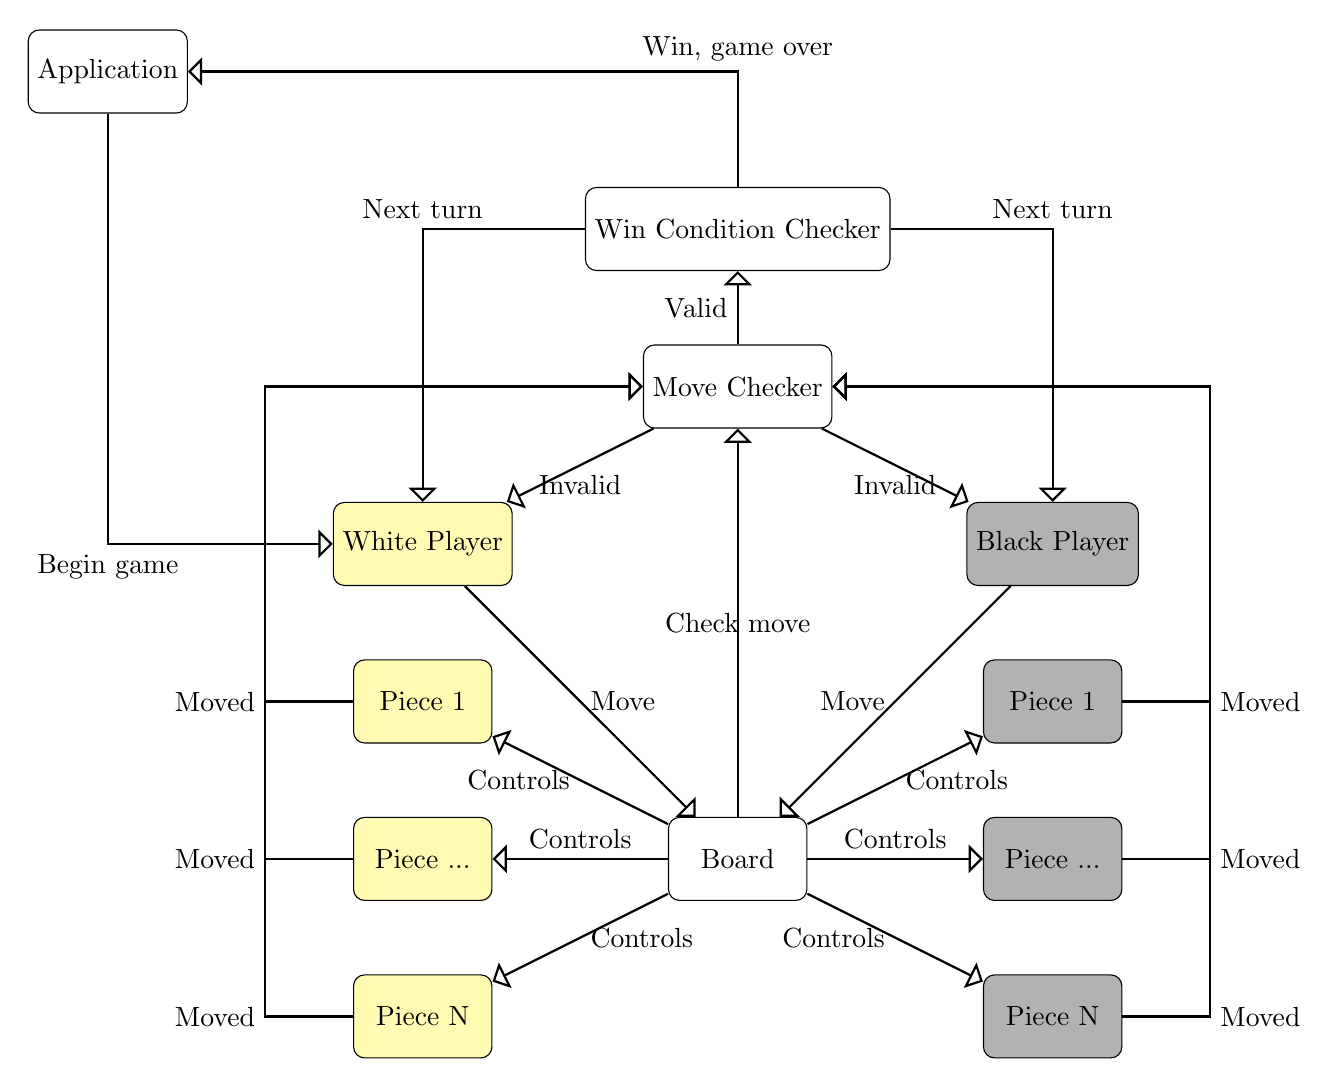
\begin{tikzpicture}
\tikzstyle{node}=[draw, rectangle, rounded corners, text centered, minimum height = 3em, minimum width=5em]
\tikzstyle{path}=[draw, ->, >=open triangle 90, thick]

\def \x {4}
\def \y {-2}
\def \offset {\x/2}

\node[node, fill=black!30]				(black) at 		(\x,			-\y)	{Black Player};
\node[node, fill=yellow!30]				(white) at 		(-\x,			-\y)	{White Player};

\node[node]								(board) at 		(0,				\y)		{Board};

\node[node, fill=yellow!30]				(wpiece1) at		(-\x,			0)		{Piece 1};
\node[node, fill=yellow!30]				(wpiece2) at		(-\x,			\y)	{Piece ...};
\node[node, fill=yellow!30]				(wpiece3) at		(-\x,			2*\y)	{Piece N};

\node[node, fill=black!30]				(bpiece1) at		(\x,			0)		{Piece 1};
\node[node, fill=black!30]				(bpiece2) at		(\x,			\y)	{Piece ...};
\node[node, fill=black!30]				(bpiece3) at		(\x,			2*\y)	{Piece N};

\node[node]								(valid) at			(0,				2*-\y)	{Move Checker};
\node[node]								(cond) at			(0,				3*-\y)	{Win Condition Checker};
\node[node]								(app) at			(2*-\x, 		4*-\y)	{Application};

\path[path] (app) |- node[below]{Begin game} (white);

\path[path] (white) -- node[right]{Move} (board);

\path[path] (board) -- node[left]{Controls} (wpiece1);
\path[path] (board) -- node[above]{Controls} (wpiece2);
\path[path] (board) -- node[right]{Controls} (wpiece3);
\path[path] (wpiece1) -| node[left]{Moved} (-\x-\offset, 2*-\y) -- (valid);
\path[path] (wpiece2) -| node[left]{Moved} (-\x-\offset, 2*-\y) -- (valid);
\path[path] (wpiece3) -| node[left]{Moved} (-\x-\offset, 2*-\y) -- (valid);

\path[path] (black) -- node[left]{Move} (board);

\path[path] (board) -- node[right]{Controls} (bpiece1);
\path[path] (board) -- node[above]{Controls} (bpiece2);
\path[path] (board) -- node[left]{Controls} (bpiece3);
\path[path] (bpiece1) -| node[right]{Moved} (\x+\offset, 2*-\y) -- (valid);
\path[path] (bpiece2) -| node[right]{Moved} (\x+\offset, 2*-\y) -- (valid);
\path[path] (bpiece3) -| node[right]{Moved} (\x+\offset, 2*-\y) -- (valid);

\path[path] (board) -> node{Check move} (valid);


\path[path] (valid) -- node[below]{Invalid} (white);
\path[path] (valid) -- node[below]{Invalid} (black);
\path[path] (valid) -- node[left]{Valid} (cond);

\path[path] (cond) -| node[above]{Next turn} (white);
\path[path] (cond) -| node[above]{Next turn} (black);
\path[path] (cond) |- node[above]{Win, game over} (app);

\end{tikzpicture}}

The game begins with white making the first move. The white player selects and moves a piece via the board, then the move is checked in the move checker. If the move is invalid then the player is asked to make a different move. In the case that the move was valid, the win condition checker verifies whether or not the win condition is satisfied, if it is then the game is over, if not then the next turn begins and the other player makes a move. Player continue making moves until the win condition is satisfied. The win condition can be satisfied if the king is in check mate, was been defeated or one of the players have disconnected from the game.

\subsection*{Question 5}
\begin{quote}
\textit{Suppose you want to provide a Web application without well defined target users. How would you ensure that your Web application works well in any browser? What should you do when a new version of a browser of released? Why?}
\end{quote}
In order to ensure compatibility the web application should be perpetually tested in all commonly used browsers. While usability testing can be confined to only testing distinct viewing platforms, i.e. mobile and pc, basic testing should be conducted to verify that everything renders as expected and that logic behaves as expected. An example of this would be launching the application in all common browsers every time new functionality has been implemented and looking for discrepancies between them. 

\subsection*{Question 6}
\begin{quote}
\textit{How would you assess the usability of your Web application?}
\end{quote}
As mentioned in the answer to question 3, a user test would be conducted.  This test would require a representative user group to undertake the test, a series of specified tasks to perform in the application and some means of measuring or monitoring the test.

The user group should be representative, this means that chess players of many different ages with different skills levels should be included. Ideally the players should also have different backgrounds to further cover possible users. In the case of Augmented Chess, non-English speaking players may be excluded since translation will not be implemented in this project.

The tasks should reflect the majority of behaviour or tasks in usage of the application. This allows us to test as much of the interface as possible. The tasks should be defined clearly and be small enough such that understanding the task is not an issue.

Finally monitoring and measurement of the tests should ideally not affect the user testing the system. This ensures greater authenticity of the results.
\subsection*{Question 7}
\begin{quote}
\textit{Can you ensure that your Web application is free of any defects? Why/How?}
\end{quote}

It is impossible to ensure that the application is completely defect free. Defects can be any number of problems with the application or the system, depending on the definition of defect. There are certain kinds of defects that are close to impossible for engineers to account for, such as an incorrectly configured browser or an operating system error on the users end. Furthermore, connectivity issues can be caused by issues outside of the engineers control.

However, web engineering can reach an adequate level of non-defection in the application. This is by maintaining a good testing strategy. Testing many browsers and different platforms allows engineers to be alerted to issues and enables them to attempt to solve them.

\subsection*{Question 8}
\begin{quote}
\textit{Propose two interesting new requirements for your Web application. Analyse the impact of those requirements in your design and implementation. Enumerate the advantages / disadvantages of changing your Web application to take them into account. Decide if you are going to do the changes and justify your decision.}
\end{quote}

The two new features this answer will discuss are a leader-board system tracking the performance of the best players and a board creator that allows players to create new asymmetrical boards to play on. Since the design of the application has been somewhat modular to support this kind of extension the main impact will be the addition of two new menu buttons for each of these features and the option to use a different type of board, when setting up a game. Furthermore, the back-end would need to keep track of the new board and the top performing players. This would require some additional data structures to represent these entities. The player performance could be represented as an attribute on the \texttt{user} data object. The leader-board then periodically collects the players performance and updates the leader-board. The board will require a new data object which encapsulates the board.

\subsubsection*{Advantages}
\begin{enumerate}
	\item Additional entertainment value
	\item Greater user/player retention
	\item Competition among players
\end{enumerate}

\subsubsection*{Disadvantages}
\begin{enumerate}
	\item Greater complexity of application
	\item Additional development complexity
	\item Greater overview difficulty
\end{enumerate}

Primarily due to the greater development complexity, these features will not be implemented into the Augmented Chess application.

\subsection*{Question 9}
\begin{quote}
\textit{Suppose that your Web application should be accessible to people with disabilities, which elements of your Web application should be adapted? How?}
\end{quote}

When answering this question we will discuss the case where a user how is unable to read or see the test attempts to use the application. This is the user which is analysed because deaf users will have no problem using the application and physically disabled individuals will have issues operating their devices, rather then the application and should there be a solution for the device operation issue, then that same solution would be applicable to the application.

The majority of the application uses alternative text for images and similar graphical elements allowing blind or dyslexic users to have the application read aloud. This is not the case with the game board however. Even if the board was properly annotated with alternative text, it would make very little sense to a blind individual if the contents of the board was simply read aloud. Instead the application should provide different textual content for the boards. Empty cells should be omitted and occupied cell information should be provided in chess notation.

\end{document}